In this section the results obtained by the face recognition algorithm is  presented. The effects of performing face detection have been ignored in these results.

Table~\ref{tb:fr_results} show the results of applying the face recognition algorithm to the test data set.

\begin{center}
  \captionof{table}{Results of performing face recognition on the test data set.}
  \label{tb:fr_results}
    \begin{tabular}{ | l | l | l | l |}
    \hline
    Number of images & False positives & False negatives & Recognition Rate \\ \hline
    78 & 0 & 10 & 86\% \\ \hline
    \end{tabular}
\end{center}

Since the LPQ method used for face recognition is supposedly blur invariant, the effects of applying different types of blur to the input images were examined to verify this claim. Figure~\ref{fig:fr_result_plots_gauss} shows how the recognition rate is effected by applying Gaussian blur to the input images while Figure~\ref{fig:fr_result_plots_motion} shows the effect caused by a linear motion blur filter.

\begin{figure}[H]
\centering
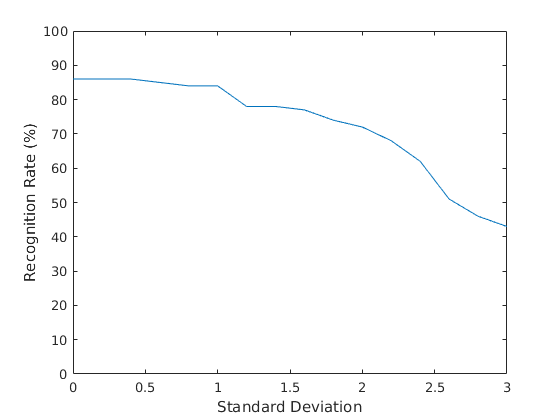
\includegraphics[width=0.62\textwidth]{img/blur_test/gauss_plot.png}
\caption{Shows how applying Gaussian blur effects the recognition rate.}
\label{fig:fr_result_plots_gauss}
\end{figure}

\begin{figure}[H]
\centering
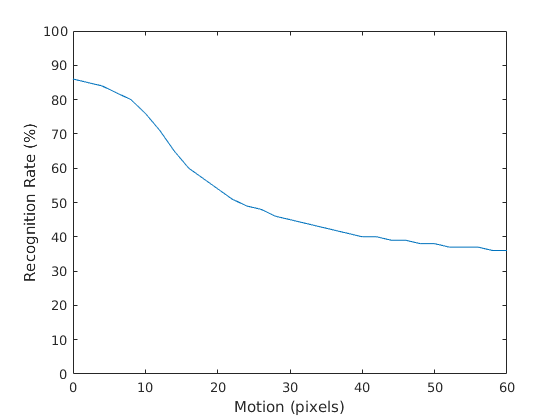
\includegraphics[width=0.62\textwidth]{img/blur_test/motion_plot.png}
\caption{Shows how applying linear motion blur effects the recognition rate.}
\label{fig:fr_result_plots_motion}
\end{figure}

Figure~\ref{fig:fr_result_plots_down} shows the result of decreasing the tone value and Figure~\ref{fig:fr_result_plots_up} shows the result of increasing the tone value.

\begin{figure}[H]
\centering
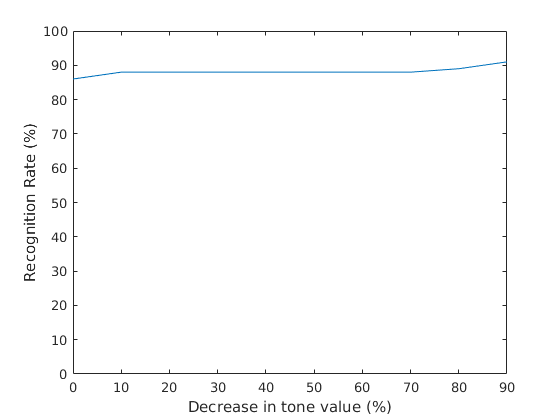
\includegraphics[width=0.62\textwidth]{img/blur_test/tone_down_plot.png}
\caption{Shows how reducing the tone value effects the recognition rate.}
\label{fig:fr_result_plots_down}
\end{figure}

\begin{figure}[H]
\centering
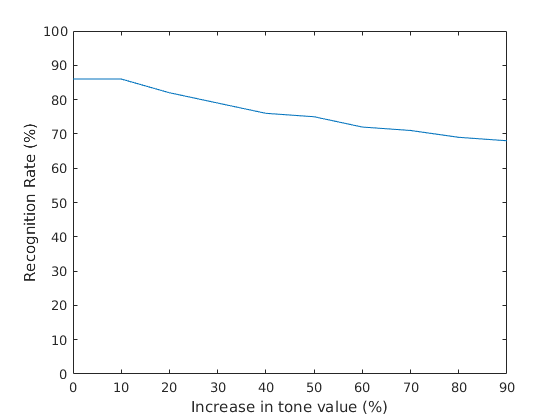
\includegraphics[width=0.62\textwidth]{img/blur_test/tone_up_plot.png}
\caption{Shows how increasing the tone value effects the recognition rate.}
\label{fig:fr_result_plots_up}
\end{figure}
